\documentclass[10pt,twocolumn, nofootinbib]{revtex4-2}

\usepackage{assumptionsofphysics}
\usepackage{tikz}
\usetikzlibrary{3d, perspective}
\usepackage{breakurl}
\usepackage{tcolorbox}
\usepackage{float}

\newcommand\mix{\mathrm{mix}}
\newcommand\component{\mathrm{comp}}
\newcommand\cospan{\mathrm{cospan}}
\newcommand\dist{\mathrm{dist}}
\newcommand\hull{\mathrm{hull}}
\newcommand\support{\mathrm{supp}}
\newcommand\capacity{\mathrm{scap}}
\newcommand\fraction{\mathrm{frac}}
\newcommand\frcap{\mathrm{fcap}}

\newcommand{\ens}[1][e] {\mathsf{#1}} % Ensemble
\newcommand{\Ens}[1][E] {\mathcal{#1}} % Ensemble space

\def\ortho{\perp}
\def\northo{\nperp}
\def\separate{\downmodels}
\def\nseparate{\ndownmodels}

\def\>{\rangle}
\def\<{\langle}

\begin{document}

\title{A non-additive generalization of probability theory \\for quantum mechanics and beyond}
\author{Gabriele Carcassi}
\affiliation{Physics Department, University of Michigan, Ann Arbor, MI 48109}
\author{Christine A. Aidala}
\affiliation{Physics Department, University of Michigan, Ann Arbor, MI 48109}

\date{\today}


\begin{abstract}
	We present a physically motivated generalization of probability theory that is suitable for classical mechanics, quantum mechanics and any future physical theory that allows a statistical description. The goal is to put the use of classical and quantum probability in a broader context, and show how the current mathematical structures are likely not suitable to solve the open problems in the foundations of physics. For the more mathematically inclined, we will point to areas where new math or generalization of established math are needed. For the more philosophically incline, we will point to areas where further conceptual work is needed.
	
	
	%Given a generic space of ensembles, we can define the fraction capacity as the maximum fraction of a particular ensemble that can be understood as a mixture of ensembles from a given set. This gives a non-additive (i.e. fuzzy) measure that reduces to a probability (i.e. additive) measure for classical spaces and for quantum measurements. We can also define the state capacity as the exponential of the maximum entropy reachable by a mixture of ensembles from a given set. This is also a non-additive measure and reduces to the Liouville measure in classical mechanics and the Hilbert space dimensions for subspaces of quantum mechanics. Conceptually, it gives us a notion of probability that is both theory and interpretation independent. Mathematically, it gives us a measure theoretic generalization of probability. Physically, it may allow to find new way to understand current theory and tool to investigate new ones. The purpose of this paper is to show the core ideas and present questions that may be developed on the mathematical, physical and philosophical side.
\end{abstract}

\maketitle

%TODO: literature search on use of signed measure in QM. ( e.g. \href{https://arxiv.org/pdf/2302.00118}{this paper})

\section{Introduction}

In the past few decades, there has been a growing interest in developing approaches that generalize the notion of states and physical theories in terms of probabilistic and/or entropic concepts, which stems from the underlying aim to characterize physical theories from an operational viewpoint. 

in terms of operations aspects, which lends themselves ,  Given the statistical/probabilistic nature of measurement outcomes and the success of information theory, a generalized notion of probability is typically assumed. . One basic insight is that statistical/probabilistic concepts often provide a suitable basis for this generalization, and it is in this setting where most of these approaches operate. A key problem, then, is what notion of probability should be used given that the standard measure theoretic Kolmogorovian approach does not generally work in quantum mechanics.

The paper aims to ask the following question: can we, by arguing from necessity, find a minimal set of physical requirements for a state space of a physical system, that allows to directly connect to all the measure theoretic structures currently used in physics (i.e. probability measures, Liouville measure to count states, quasi-probability, ...) and point to a straight-forward generalization of such structures? We will show that this is indeed possible.\footnote{Note that we believe that the requirements we set, though necessary, are not sufficient to generalize the Lie algebra given by the classical Poisson brackets and the quantum commutators, meaning they cannot fully recover mechanics. Nonetheless, they are enough to recover measure theoretic structures, the topic of this paper.}

The starting point is that any physical law deals with experimentally reproducible relationships. This implies a physical theory must gives us the space of statistical ensembles (i.e. the collection of all possible preparation procedures) that the theory allows. As a basic requirements, ensembles must be experimentally well-defined (leading to a topological space), allow statistical mixing (leading to a convex structure) and quantify the variability of the elements of the ensembles (leading to an entropy function).\footnote{The main point of departure from GPTs is the entropy requirement. We found that a convex set is not enough to fully characterize an ensemble space, especially in the infinite dimensional case.} Additionally, though not necessary, we require having enough real valued quantities to identify each ensemble (leading to the continuous embedding into a Hausdorff locally convex topological vector space). Mathematically, under these premises, an ensembles space is a convex subset of a locally convex topological vector space. The question is, then, what measure theoretic tool can quantify the number of states (as in the classical Liouville measure) or the number of possible outcomes of a measurements (as in the dimension of orthogonal subspaces of an operator)? What measure theoretic tool can represent each ensemble? If we are to define a physically meaningful notion of probability density, both of these questions must be answered.

We will first review how measure theory is used in classical probability together with some results from Choquet theory. This will tell us that elements of a compact convex set can always be represented by a probability measure over its extreme points, the pure states. While such representation is always possible, at least in the compact case, it is not unique. Uniqueness requires the space to be a Choquet simplex, which is a generalization of the standard finite-dimensional simplex and represents the classical case. The key insight, then, an ensemble space is classical if and only if each ensembles admits a unique decomposition in terms of pure states.

We will then review some results from the use of quasi-probability measures. While the Wigner function represents the most known instance, there are different choices depending on the problem at hand. The key insight is that it is not negative probability that characterizes quasi-probability, but the lack of mutual exclusivity of the points of the space. The quasi-probability measures, in fact, are not defined over the extreme points, but over a suitable set $K$ such that the space of signed probability measures is isomorphic as a vector space to the one that embeds the ensemble space. Therefore, while signed measures are a powerful tool for calculation in specific problems, they cannot give us a general principled representation of the physical theory.

The above two approaches exhaust what can be done with additive measures, so we turn to the non-additive case. Given an ensemble $\ens$, we can ask what fraction can be produces by a mixture of a given ensembles. This leads to the fraction capacity: a sub-additive set function that, like the probability measure, is bounded to one, monotonic and continuous from above and below. Over the extreme points, the fraction capacity represents the supremum of all possible measures that can represent the same ensemble in Choquet theory. The classical case exactly corresponds to the simplex case, in which fraction capacity corresponds to a unique measure, and is therefore additive. This again solidifies the connection between classical probability, additivity of measure and mutual exclusivity.

We can also generalize a notion of count of states. While in classical statistical mechanics we start with a measure that quantifies the count of states and define the entropy using its logarithm, for the ensemble space we proceed in the opposite way: we start from the entropy and we define the count of states as the exponential of the entropy (i.e. the entropic volume). From this, we can define a state capacity, which is again a sub-additive measure. It reduces to the Liouville measure in the classical case and the dimensionality of the Hilbert space in the quantum case.

Lastly, we lay down the requirements for a non-additive generalization of probability theory. While should be in principle possible, we show that the most used non-additive integral, the Sugeno and Choquet integral, do not work for our purposes. This means that more work will be needed to develop the appropriate tools.

A final remark before we start. Too often works in the foundations of physics focus on a particular aspect without concern to a broader connection to all relevant mathematical, physical and philosophical aspects. Therefore, it is important to us that this work is a piece of a much larger puzzle, which connects cleanly and directly to  other areas, such as information geometry, functional analysis, quantum logic and so on. It is the hallmark of a true fundamental structure for physics that such connections can be easily made. Unfortunately, the nature of scientific publication requires us to publish a narrow slice of the work to fit the scope of a particular journal. Ironically, this means that the most important motivations for our approach are out of scope of this article, as we will concentrate only to the connections to measure theory.

\section{Ensemble space}

\textbf{Basic requirements for an ensemble space}. It is a cardinal rule in Physical Mathematics that all axioms and mathematical definitions must be grounded in physical requirements. This way we can develop mathematical frameworks that are physically well founded. As part of our larger project, we are developing a general theory of ensemble spaces, the full treatment of which is beyond the scope of this work. We limit ourselves to give the initial premises and the final mathematical characterization, without justifications and proofs.\footnote{More details are available in our ongoing work (cite)}

We start by assuming that physical laws deal with experimentally reproducible relationships, which implicitly requires the notion of statistical ensembles. Conceptually, a statistical ensemble is the collection of outputs, taken at once, of a reproducible preparation procedure for a physical system. In the classical case, this corresponds to a probability distribution over a discrete set of outcomes (e.g. a fair coin) or over phase space (e.g. the symplectic manifold representing position and momentum for a classical particle). In the quantum case, this corresponds to a mixed state (e.g. a positive semi-definite self-adjoint operator of trace one). A physical law, then, ultimately expresses relationships among ensembles. A minimal requirement for a physical theory, then, is to provide an ensemble space: the collection of all possible ensembles within the theory, together with a basic mathematical structure that all physical theories must possess.

An ensemble space $\Ens$ will need to satisfy three basic requirements. First, it needs to guarantee experimental verifiability. Mathematically, the ensemble space must be a $\mathsf{T}_0$ second countable topological space, where each open set represents an experimentally verifiable statement.\footnote{A verifiable statement is an assertion for which there exists an experimental test that finishes successfully in finite time if and only if the statement is true.} Second, it needs to allow statistical mixtures: if $\ens[a],\ens[b] \in \Ens$ are ensembles, then $p \ens[a] + \bar{p} \ens[b]$ represents the statistical mixture where $\ens[a]$ is taken with probability $p$ and $\ens[b]$ with probability $\bar{p} = 1 - p$. Mathematically, this constrains the ensemble space to be a convex set.\footnote{Only finite mixtures are guaranteed, while the topology will decide whether an infinite mixture $\sum_{i}^{\infty} p_i \ens_i$ converges in the space or not.} Third, an entropy function must be defined that characterizes the variability of the elements within an ensemble.

Additionally, we will require that ensembles can be identified through real valued statistical quantities.\footnote{It is an open question whether this is an additional assumption or it can be derived from the other requirements.} A statistical quantity represents the expectation of a real valued quantity, and is therefore an affine continuous function $F : \Ens \to \mathbb{R}$. That is, $F(p \ens[a] + \bar{p} \ens[b]) = p F(\ens[a]) + \bar{p} F(\ens[b])$. The last requirement is that there exists a family $F_i$ of statistical quantities that fully identify each ensemble. That is, $F_i(p \ens[a] + \bar{p} \ens[b]) = p F_i(\ens[a]) + \bar{p} F_i(\ens[b])$ and $\ens[a] = \ens[b]$ if and only if $F_i(\ens[a]) = F_i(\ens[b])$ for all $i$.\footnote{For example, on the continuum this means that the moment problem is solvable: you can identify the distribution by the expectation of the polynomials of position and momentum. Similarly, in quantum mechanics means that the state can be reconstructed through quantum tomography.}

Each physical theory satisfies these axioms, even though it may be represented very differently mathematically. Classical mechanics, for example, is typically described in terms of the geometry of phase space. Quantum mechanics is most often defined in terms of complex inner product spaces, but can be reframed in terms of quasi-probability distributions. Therefore, while the above requirements are needed for a physical theory, it does not necessarily mean that it is convenient to describe problems or make calculations in terms of those definitions. In fact, those requirements interact with each other leading to a rich mathematical structure that connects to many of the structures we use in mathematical physics, and its goal is mainly to see how the different representations are connected.

The goal of this paper is to examine the different ways that measure theory can be used to represent ensembles in any given physical theory.

% space is metrizable https://proofwiki.org/wiki/Birkhoff-Kakutani_Theorem/Topological_Vector_Space

\textbf{Ensemble spaces as convex sets.} For the purpose of measure theoretic representations, it is best to understand an ensemble space $\Ens$ as a convex subset of a metrizable second countable locally convex topological vector space $V$.\footnote{The entropy constraint forces the topology to be $\mathsf{T}_1$ the convex space to embed into a vector space. A second countable $\mathsf{T}_1$ TVS is metrizable. The family of statistical quantities induces a family of semi-norms on the space, which must be countable due to second countability, which makes the TVS locally convex.} The entropy is a function $S : \Ens \to \mathbb{R}$ that satisfies the following bounds
\begin{equation}
	\begin{aligned}
		p S(\ens[a]) + (1-p) &S(\ens[b]) \leq S(p \ens[a] + (1-p) \ens[b]) \\
		&\leq I(p,\bar{p}) + p S(\ens[a]) + (1-p) S(\ens[b])
	\end{aligned}
\end{equation}
where $I(p,\bar{p}) = - p \log p - \bar{p} \log(\bar{p})$.\footnote{In the larger work, we can show that the Shannon entropy is the only upper bound possible.}  Intuitively, the variability (i.e. the entropy) cannot decrease during mixing, and will have an upper bound when mixing two ensembles whose instances are always distinguishable.

Using the convex structure, we say that two ensembles are separate, noted $\ens[a] \separate \ens[b]$, if they cannot be expressed as a mixture of a common ensemble. That is, there is no $\ens[c]$ such that $\ens[a] = \alpha \ens[c] + \bar{\alpha} \ens[d]$ and $\ens[b] = \beta \ens[c] + \bar{\beta} \ens$ from some $\alpha, \beta \in (0,1]$ and $\ens[d],\ens \in \Ens$. No ensemble is separate from itself. An internal point is an ensemble that is not separate from any ensemble (i.e. it is the mixture of any ensemble). An extreme point is an ensemble that is separate from all others (i.e. it is only a mixture of itself).

TODO: figure with classical triangle and quantum Bloch Ball

The set of all extreme points $X$, as we will see, plays a major role. However, on physical grounds, these may not be proper ensembles. In classical mechanics, these would correspond to Dirac measures: probability distributions all concentrated at a single point of phase space. Since we cannot reliably prepare a particle with infinite precision, and its entropy would correspond to minus infinity, these are not ensembles and they are not part of $\Ens$. For the purpose of Choquet theory, we will assume that there is a way to find the closure $E \supset \Ens$ that includes all extreme points $X$. Moreover, we will also assume $E$ to be compact, even though it will not be in general. How to properly make these identifications, and how to go beyond the compact case, is outside of the scope of this particular article.\footnote{An early attempt used the notion of orthogonality to create the lattice of orthogonal subspaces and use something along the lines of Stone's representation theorem for Boolean algebra. This does not work. An approach, currently under investigation, is to study limits over statistical quantities. We are still trying to understand what mathematical structures have enough information to allow the reconstruction.} Note that the classical discrete and the quantum case fall in the compact case. Moreover, the set of all probability distributions over a compact space $X$ also falls in the compact case. Therefore, apart from the technicality above, the compact case is still a very interesting case. To distinguish the context, in this article we will use $\Ens$ to indicate the general case and $E$ to indicate this ``compact closure.''

\textbf{Orthogonality and separatedness.} We will say that two ensembles are orthogonal, noted $\ens[a] \ortho \ens[b]$, when their mixture gives a maximal entropy increase. This will recover the notion of orthogonality for both classical and quantum spaces. Conceptually, these correspond to two ensembles where all instances are distinct from the other: they are mutually exclusive and a single instance is enough to distinguish between the two cases. 

In classical spaces, orthogonality and separatedness coincide: two ensembles are orthogonal and separate if and only if the support of the respective probability distributions overlap on a non-measure-zero set. In quantum mechanics, these two notions are different: any two pure states are separate but are not orthogonal. For example, pure ensembles of spin up and spin down are orthogonal, mutually exclusive, precisely because it takes one instance to determine which one is which. Pure ensembles of spin up and spin right, however, are not orthogonal precisely because, in some cases, their instance cannot be perfectly discriminated. They are, however, orthogonal, because they are both pure states, one is not the mixture of other ensembles: they are extreme points.

It is the ease with which such distinctions between the classical and quantum case can be made that is the main appeal for this structure. We will see over and over how mutual exclusivity is linked to classical probability and its failure in quantum, and other non-classical, theories.

To summarize, a repeatedly verifiable physical theory requires ensembles, which must be defined experimentally, allow statistical mixing and provide an entropy. Additionally, we require the existence of enough statistical quantities to identify each ensemble. Under these assumptions, an ensemble space $\Ens$ is a convex set of a metrizable second countable locally convex topological vector space $V$. In some cases, for simplicity, we will require $\Ens$ to admit a ``compact closure'' $E$, so that it includes the set $X$ of its extreme points. We now turn to the question of how we can represent both the entropy and each ensemble in terms of some measure theoretic structure.

\section{Probability measures and Choquet theory}

\textbf{Classical probability measures.} In the classical case, given the topological space of possible states $X$ (i.e. the sample space), ensembles are defined as probability measures $p : \Sigma_X \to [0,1]$. That is, a probability measure assigns to each element of the Borel algebra $\Sigma_X$\footnote{In our overall project, Borel sets represent statements associated to a test, regardless of termination.}, an event, the probability to find it to be true. In the discrete case, like for roll of a die, $X$ is a set endowed with the discrete topology\footnote{Physically, the discrete topology corresponds to the ability to experimentally verify or falsify each case. That is, we are able to recognize whether a particular die landed or didn't land on a particular face.} and, consequently, the power set is the $\sigma$-algebra. In the continuous case, $X$ will be classical phase space endowed with the usual topology of a manifold.\footnote{Physically, the topology of a manifold corresponds to the ability to label each possible case through a set of continuous variables which are verifiable up to finite but arbitrarily small precision.}  The probability measure is countably additive, meaning that, given a countable collection $A_i$ of pair-wise disjoint events (i.e. $A_i \cap A_j = \emptyset$), the probability of the union is the sum of the probability of the respective events:
\begin{equation}
	p\left(\bigcup_i A_i \right) = \sum_i p(A_i).
\end{equation}
This last requirement codifies the idea that disjoint events are mutually exclusive: if $A$ and $B$ cannot happen at the same time, then the probability of one of the two happening is the sum of them separately happening.

\textbf{Expectation and integration.} A random variable is a function $F : X \to \mathbb{R}$ that assigns a value to each state.\footnote{The function $f$ must be measurable, in the sense that the inverse of a Borel set should be a Borel set. We find that the term is confusing for a physics audience, so it is avoided in the main text.} The number of the side of the die, position, and momentum are typical examples. The expectation for a random variable is given by the integral
\begin{equation}
	E[F] = \int_X F dp.
\end{equation}
The expectation is linear with respect to the variable (i.e. $E[aF+bG]= aE[F]+bE[G]$). In our case, what is more interesting is that it is a convex function in terms of probability measures: if $p = \lambda p_1 + \bar{\lambda} p_2$ then $\int_X F dp = \lambda \int_X F dp_1 + \bar{\lambda} \int_X F dp_2$. That is, as we required for statistical variables, the expectation for a mixture is the mixture of the expectations.

\textbf{Absolute continuity of probability measures.} As we saw before, probability measures over a single point over the continuum cannot be understood as valid ensembles. To address this, we add a requirement that is both physically meaningful and mathematically useful. Let $\mu : \Sigma_X \to [0, + \infty]$ be a measure on $X$ that quantifies the count of states in each region. In the discrete case this is simply the counting measure (i.e. three possible faces of the die correspond to three possible states), while in the continuous case this corresponds to the Liouville measure (i.e. volumes in phase space correspond to the count of states). This measure is additive over disjoint regions as they represent mutually exclusive events. The requirement is that we can assign non-zero probability only to events that have a non-zero count of states. That is, if for a particular event $A$ we have $p(A) \neq 0$, then we must have that $\mu(A) \neq 0$ as well. Mathematically, $p$ is absolutely continuous with respect to $\mu$, and this is exactly the case in which a probability density $\rho = \frac{dp}{d\mu}$ can be defined.\footnote{In the general case, we can still assign non-zero probability to a point of a manifold, provided that the topology and the measure $\mu$ consistently allow for it. Physically, it means that those points are ``special'' both in terms of experimental verifiability and entropy/count of states. While the general framework allows for it, it is not crucial for our discussion here.} This is another example in which a physical requirement (probability must be zero if there are no possible states), once properly spelled out (absolute continuity), justifies common physical intuition (we assume a probability density exists).

\textbf{Choquet theory.} Classical statistical mechanics and probability start by assuming the existence of a state space $X$ and defining ensembles on top of it. This cannot be generalized to quantum mechanics and beyond. In our theory of ensemble spaces we start with ensembles, and have to show when and how they can be thought, can be represented, as probability measures. If we can assume that $E$ is a compact convex set, Choquet theory answers this question.

First, we have to define what it means to represent an ensemble with a probability measure. Let $E$ be a convex subset of a locally convex space $V$ and $X$ the set of extreme points. In classical mechanics, $X$ will correspond to the set of Dirac measures, as these cannot be seen as a mixture of other measures. In quantum mechanics, $X$ corresponds to the pure states, as these cannot be seen as a mixture of other states. In other words, the set of states $X$ is recovered as the set of ensembles with the narrowest spread. We say that $\ens \in E$ is represented by a probability measure $p : \Sigma_{E} \to [0,1]$ if $f(\ens) = \int_E f dp$ for every continuous linear functional $f$ on $V$. Moreover, $p$ is supported by the extreme points if $p(X) = 1$. Physically, we start with an ensemble $\ens$ taken as a point in our ensemble space, identified by the value of all possible statistical variables $f(\ens)$, and we represent it as a probability measure $p$, a statistical mixture, over other the extreme points, the states, recovering the expectation with an integral.

We should note that, given any probability measure $p$ over the extreme points $X$, we can always find an $\ens \in E$ that is represented by $p$. Therefore, we have a map from the set of probability measures to the set of ensembles. The first question, then, is whether we can go back. Choquet theory tells us that, in the compact case, we can:
\begin{thrm}[Choquet 1]
	Let $E$ be a metrizable compact convex subset of a locally convex space $V$, and let $\ens \in E$. Then there exists a probability measure $p_{\ens}$ on $X$ which represents $\ens$ and is supported by the extreme points $X$.
\end{thrm}
Note that an ensemble space is a metrizable convex subset of a locally convex TVS. Therefore, if $E$ is compact, the Choquet theorem applies.

The above theorem tells us that the map between probability measures and ensembles is surjective. The second question, then, when is it bijective? Again, Choquet theory has a clear answer.
\begin{thrm}[Choquet 2]
	Let $E$ be a closed convex metrizable subset of a locally convex space $V$. Then $E$ is a Choquet simplex if and only if for each $\ens \in E$ there exists a unique measure $p_{\ens}$ which represents $\ens$ and is supported by the extreme points $X$.
\end{thrm}
The Choquet simplex is a generalization of the finite dimensional simplex, whose mathematical characterization is rather technical. The key point is that $E$ is a Choquet simplex if and only if the ensemble space does not allow multiple decomposition in terms of pure states. This confirms the physical intuition from classical and quantum statistical mechanics.

For example, the ensemble space for a two state quantum system, the Bloch ball, is a compact convex subset. Any internal point can be seen as the convex combination of points on the surface, the pure states. The center, which represents the maximally mixed state, can be thought as an equal mixture of any two opposite points, or a uniform distribution over the whole surface. The fact that any ensemble can be seen as a mixture of a set of pure states, then, is reflected by the first part of the Choquet theorem, and it is valid for all physical theories. Uniqueness of the representation fails, however, precisely because the ensemble space is not a simplex: it is not a classical space.

The core insight from Chouqet theory, then, is that both in the classical and quantum case we can represent ensembles as a probability distribution over a set of states. However, only in the classical case this representation is unique. In the quantum case, mixed states can be decomposed into pure states in multiple ways, and it is this multiple decomposition that makes the ensemble space not a simplex, and therefore the space not classical. Unique representation of ensembles is a desirable property, and standard probability measures are not going to provide it in general.

\section{Quasiprobability}

%Goal of this section: quasi-probability representations are allowed by the embedding in a topological vector space. Choice of representations are guided by what observables are interesting for a specific problem.

%Examples: Wigner, Husimi, Glauber P, SIC-POVM (space not made of spectra of operators), Kirkwood-Dirac (two-time correlation function - observables not necessarily taken at the same time )

%Things to say: some people think about it as weakining axioms (cite papers on negative probability). It's more than that. Points describe events that are not necessarily mutually exclusive. TODO: example of two Wigner function/Husimi Q would be better that have no overlap but they are not orthogonal and/or two functions that have overlap but are orthogonal.

%Thing to say: all these representations are useful because they preserve the linear structure, meaning that convex combinations of ensembles are convex combinations of quasi-probability; expectation values are linear. Check, but it should be true.

% 1 describe quasiprobability approaches; go through examples; point out that the quasi-probability can be negative; that one can recover expectations;

\textbf{Quasi-probability representations.} Another way to represent quantum ensembles is through the use of quasiprobability distributions, of which the Wigner function is probably the most widely known. The Wigner transform $W : \Ens \to L^1(\mathbb{R}^2, \mathbb{R}) $, defined as \cite[eq.~11.8-3a]{mandel1995}
\begin{equation}
	W(\rho) = W_{\rho} (q, p) = 2 \int_{-\infty}^{\infty} \langle x + y | \rho | x - y \rangle e^{-2 i p y / \hbar} \; \mathrm dy,
\end{equation}
takes a mixed state $\rho$ and returns a real function $W_{\rho}$ of phase space that, like a probability density integrates to one, but, unlike a probability density, can be negative. Recall that an affine combination is a linear combination where all coefficients sum to one but are not necessarily non-negative. Therefore, in general, quasi-probability distributions can be understood as affine combinations. Remarkably, expectation values of polynomials of position and momentum in symmetric ordering coincide with expectations over the Wigner function. For example
\begin{equation}
	\tr \left( \frac{1}{2}[XP+PX] \rho \right) = \int_{-\infty}^{\infty} \int_{-\infty}^{\infty} xp \; W_{\rho} (q, p) dq dp \; .
\end{equation}
Moreover, the transform is an affine map: $W(p \rho_1 + \bar{p} \rho_2 ) = p W(\rho_1) + \bar{p} W(\rho_2)$.

In some problems, especially in quantum optics, normal ordering and anti-normal ordering are more useful. The Glauber P representation and the Husimi Q representation work like the Wigner function except that the expectations of polynomials recover the respective order. In other circumstances, quasi-probability distributions over observables different from position and momentum are more useful. For example, the Kirkwood-Dirac is used to represent two-time correlation functions over observables defined at different times \cite{lostaglio2023}. Quasi-probability representations are also used over discrete elements that may not even correspond to eigenstates of a particular operator. For example, the SIC-POVM represents quantum states as affine combinations of pure states $P_i$ that are ``equally distant'' from each other, which means that no two elements are orthogonal to each other. Each ensemble $\rho$ can then be represented as \cite[eqs. 28-29]{fuchs2004}
\begin{equation}
	\rho = \sum_{n=1}^{d^2} \lambda_i P_i = \sum_{n=1}^{d^2} \left[ (d^2 + 1) p_i - \frac{1}{d} \right] P_i \; ,
\end{equation}
where $p_i = \tr \left(P_i \rho\right)$.

It should be clear that there are many ways to represent quantum states via quasi-probability distributions, and that the choice of representation is a matter of convenience for the problem at hand. All representations, though, have the following features in common. First, we have a map $W : \Ens \to Q(Z,\mathbb{R})$ that given each mixed state $\rho \in \Ens$ returns the corresponding quasi-probability function $w(z) \in Q(Z,\mathbb{R})$, where $Q(Z,\mathbb{R}) \subset L^1(Z,\mathbb{R})$ is the function space used by the specific representation. The space $Z$, in fact, can change from representation to representation: it is $\mathbb{R}^{2n}$ for a Wigner function, $\mathbb{C}^n$ for the Husimi Q and $[1, d^2] \subset \mathbb{N}$ for the SIC-POVM. All representations preserves convex combinations: $W(\sum_i p_i \rho_i) = \sum_i p_i W(\rho_i)$. That is, a statistical mixture of quasi-probability distributions represents the statistical mixture of the corresponding states. Since the map is linear, and expectation values are linear, one can express expectation values as integrals or sums over the quasi-probability $w(z)$. 

% 2 Note that it's not about negative probability; disjoint not mutually exclusive

\textbf{Not about negative probability.} The inclusion of negative probability is often advertised as the main difference between classical probability and quasi-probability \cite{adhikary2020}. Sometimes these negative probabilities are justified as arising from constraints on probability distributions defined on different contexts. This is a mischaracterization. For example, the Husimi Q representation provides us with a non-negative quasi-probability function. That is, the Husimi Q is a non-negative density distribution that integrates to one, yet it is not a classical probability distribution.\footnote{Since the Husimi Q is defined as $Q_{\rho} ( \alpha ) = \frac{1}{\pi} \langle \alpha | \rho | \alpha \rangle$, it is proportional to the probability of measuring a coherent (i.e. Gaussian state) $| \alpha \rangle$, which is non-negative. } Similarly, a SIC-POVM characterizes the Bloch ball by four pure states that form a tetrahedron inscribed in the ball. Since we can also inscribe the Bloch ball inside a tetrahedron, we can represent all states of a two-state quantum system by a convex combination of the vertices, leading to a non-negative quasi-probability distribution over four elements.

Conversely, we can use signed measures to represent classical distributions. Suppose we have a two state classical discrete space, which means the space of all possible ensembles is spanned by $[p, (1-p)]$. Alternatively, we can write it as $p[1,0] + (1-p)[0,1]$ which highlights that we are writing each possible probability distribution in terms of the two possible cases. But we could also express each probability distribution in terms of other two distributions, as in $\left(2p - \frac{1}{2}\right)\left[\frac{3}{4}, \frac{1}{4}\right] + \left(\frac{3}{2} - 2p\right)\left[\frac{1}{4}, \frac{3}{4}\right]$. The coefficients now span between $\left[-\frac{1}{2}, \frac{3}{2}\right]$, can be negative, but still sum to one. That is, in terms of this new affine basis, we need to use a signed probability.

Since we can represent classical states with signed probability measures, and quantum states with non-negative probability measures, the difference between classical probability and quantum quasi-probability does not lie in the use of negative probability. Instead, the crucial difference is that in classical probability all points of the sample space, and therefore disjoint regions, represent mutually exclusive events, and all mutually exclusive events are represented by disjoint regions. Mutually exclusive events can be prepared and observed independently from the others (i.e. they are orthogonal in the sense that they maximize entropy increase during mixture); we can assign some probability to some region without having to assign it to another disjoint region.\footnote{The only constraint is that the probability over the whole space is one.} This is not the case for quasi-probability in quantum mechanics.

For example, given a pure state $|\psi\>$, the Husimi Q function representing it is given by $Q_\psi(\alpha) = \frac{1}{\pi} |\langle \alpha | \psi \rangle|^2$. The inner product is given by \cite[eq. 11.7-1]{mandel1995}
\begin{equation}
	\langle \alpha | \psi \rangle = e^{-|\alpha|^2/2} F_\psi(\alpha^\ast)
\end{equation}
where $F_\psi$ is an entire analytic function, which cannot vanish on an open set without vanishing everywhere, therefore the support of all Husimi Q functions is the whole space $Z$. This means that orthogonal states, which correspond to mutually exclusive events in quantum theory, always have the same support; moreover disjoint subsets of $Z$ cannot be thought of as mutually exclusive events because we are not going to be able to find two distributions with those subsets as their respective supports. For the discrete case, a SIC-POVM representation picks $d^2$ pure states $P_i$ in a $d$ dimensional space, which means they cannot all be orthogonal to each other. For a Bloch sphere, the four corners of the tetrahedron are not all opposite to each other. Therefore, disjoint sets of $P_i$ do not correspond to mutually exclusive events. Quasi-probability representations, then, fail to be true probabilities not because of negative values, but because the points of the space do not represent mutually exclusive events.

% 3 These representations are possible because of the vector space structure of the ensemble space, and therefore something similar will be possible in ANY physical theory

\textbf{Ensemble space embedding and signed measures.} We saw that negative probability is a red herring, and mutual exclusivity is key. But how exactly does mutual exclusivity give us classical probability? Moreover, are quasi-probability representations specific to quantum mechanics, or are they more general? This is where the perspective from the ensemble space framework allows us to answer these questions directly.

In Choquet theory, we saw that classical spaces, Choquet simplexes, are those in which there is a one-to-one correspondence between probability measures and ensembles, where no multiple decomposition in terms of pure states is allowed. We want to show that this is a consequence of assuming mutual exclusivity between the points of $X$. Suppose we have an ensemble $\ens$ that can be represented as different measures $p_1$ and $p_2$ over the extreme points. This means that there are two disjoint sets $A, B \subseteq X$ for which $p_1(A) < p_2(A)$ and $p_1(B) > p_2(B)$. That is, we can move probability from $A$ to $B$ while leaving the ensemble, and therefore the entropy and all statistical variables, unchanged. If $A$ and $B$ were two mutually exclusive events, this would not be possible: if we could distinguish between $A$ and $B$, something would have to change. The only way for $A$ and $B$ to be mutually exclusive, then, is if different measures represent different ensembles, which means the ensemble space is a simplex. This tells us that we can use classical probability exactly when all extreme points are mutually exclusive (i.e. orthogonal as defined from the entropy) and the ensemble space is a simplex.

That is, classical probability does not merely correspond to the use of a single non-negative probability measure. It corresponds to the ability to, conceptually, allow any possible probability measure to describe a possible distinct scenario. This requirement is exactly mutual exclusivity. In quantum mechanics, a classical context is a simplex embedded within the ensemble space. For the Bloch ball, a classical context is an axis that connects two opposite points. The points are orthogonal because the midpoint is the maximally mixed state, which therefore maximizes the entropy increase, and the line segment is a one simplex. If we take the position operator and consider all density operators that commute with $x$, this is corresponds to the set of functions $\rho(x)$ that integrate to one, which is the space of probability supported by $X$, which is a simplex.

Now the second question: why does quantum mechanics allow quasi-probability representations? Let $Z$ be the space over which we are defining our quasi-probability distributions. Note that, in general, $Z$ is not the space of states. Wigner functions, for example, are defined over phase space, which does not represent quantum states. Let $M^{\pm}(Z)$ be the space of all bounded signed measures over $Z$. Since the linear combination of two bounded signed measures is a bounded signed measure, $M^{\pm}(Z)$ is a vector space. Now let $M_1^{\pm}(Z)$ be the space of signed probability measures. While it is not a subspace of $M(Z)$, it does not include the zero measure, it is an affine subspace therefore, up to the choice of an arbitrary origin, it is a vector space.

Recall that an ensemble space must be a convex subset of a vector space. If we are able to represent ensembles as quasi-probability distributions over $Z$, then, $M_1^{\pm}(Z)$ will be isomorphic to the embedding vector space $V$ as topological vector spaces.\footnote{The question of whether such an $Z$ always exists is still open for us. A possible conjecture is that $Z$ could be constructed from the statistical quantities $F_i$ that fully identify each ensemble in $\Ens$.} In this case, any element $v\in V$ can be represented uniquely by a signed probability measure $\mu_{v}$, regardless of whether it is an actual ensemble or not. Since statistical quantities $F_i$ are linear functional, we will have $F_i(v) = \int_Z F_i(z) d\mu_{v}$. In other words, there is nothing special about quantum mechanics that allows quasi-probability representations. It is the fact that the ensemble space embeds into a vector space, a general fact for all theories, that allows such representations.

It should be clear that, since an ensemble space is a strict subset of the embedding vector space, not all affine measures will correspond to an ensemble space. Whether all probability measures correspond to a valid ensemble, or whether signed probability measures are even used depends on how the mapping is done in each particular case. For example, there is no simple characterization of which Wigner functions correspond to valid quantum states and which do not.

% 4 pros and cons - can choose a repretation for the problem at hand; no fundamental representation; boundaries ore not well defined (i.e. which functions represnt valid states)

\textbf{Non-uniqueness of quasi-probability.} Our approach gives us a consistent view of both quasi-probabilities and classical probability. The first are affine representations of the ensembles that connect to the vector space structure, while the second are convex representations of the extreme points which rely on the shape of the ensemble space.

Quasi-probability distributions are very useful in practice, particularly because one can construct them to fit particular problems. Once one has identified a set of observables that are the most natural ones to define a problem, one may find a representation that is specifically suited for the case. While the quasi-probability cannot be interpreted as probability, it still provides a useful tool to describe and understand the problem and give some intuition.

However, this practical convenience is also a drawback for finding a more general approach to probability in spaces beyond classical mechanics. Crucially, the space $Z$ over which the quasi-probability measures are defined is not unique, and it is not defined by the structure of the ensemble space and, as a consequence, cannot tell us which quasi-probability measures represent valid ensembles and which do not.

As a comparison, in the previous case all probability measures were given over a uniquely defined set of points, the extreme points of the ensemble space, but the probability measure may not be unique. In this case, the quasi-probability associated to each ensemble is unique, but the space over which the quasi-probability is defined is not.

\section{Fraction capacity}

\textbf{Probability of outcomes vs fraction of components.} We saw that classical probability fails in quantum mechanics because pure states are not always mutually exclusive, are not orthogonal. That is why, in quantum mechanics, probability can be defined only once a context, an orthogonal basis, is chosen. Therefore, at a conceptual level, probabilities can only give us a patchwork representation of ensembles. Some authors embrace this view, by characterizing states as the collection of all probability distributions of all possible results, each distribution providing partial information. [CITATION NEEDED] However, there is a different route.

Note that the linearity in our axioms is in terms of mixing coefficients, not probability of outcomes. That is, regardless of whether we can characterize experiment outcomes with probability distributions, preparation procedures will always allow us to create a statistical mixture. As we saw in Choquet theory, the difficulty is that there are multiple ways to mix pure states to recover the same ensemble. However, the question of what is the biggest mixture coefficient one can use in a specific case is well-defined, and generalizes to the non-compact case as well. Therefore, our generalization of probability is not in terms of what an ensemble can lead to (i.e. measurements), but in terms of how ensembles can be produced (i.e. preparations).

\textbf{Fraction capacity.} Let us concentrate on the following problem: given an ensemble $\ens \in \Ens$ and a (Borel) set of ensembles $A \subseteq \Ens$, what fraction of $\ens$ can be constructed by a mixture of $A$? How much of $\ens$ can be explained as coming from preparations corresponding to $A$? For example, let $\Ens$ be the space of all probability distributions for a six-sided die. Let $\ens_{123456}$ be the uniform distribution over all outcomes. Let $A_1 = \{\ens_1\}$ where $\ens_1$ represents outcome one with 100\% probability. Since we can write $\ens_{123456} = \frac{1}{6} \ens_{1} + \frac{5}{6} \ens_{23456}$, where $\ens_{23456}$ represents a uniform distributions over the five outcomes, $1/6$ of $\ens$ can be constructed from $A$, but no more. Similarly, if $A_{12} = \{\ens_{1},\ens_{2}\}$, we can write $\ens = \frac{1}{3} \left(\frac{1}{2} \ens_1 + \frac{1}{2} \ens_2 \right)  + \frac{2}{3} \ens_{3456}$, so $1/3$ of $\ens$ can be constructed from $A$, but no more. Note that, given the uniform distribution, $1/6$ is exactly the probability for the event $A_1$ and $1/3$ the probability for event $A_{12}$. This gives the basic insight for our definitions.

Given a target ensemble $\ens \in \Ens$ and an arbitrary ensemble $\ens[a] \in \Ens$, we define the \textbf{fraction} of $\ens[a]$ in $\ens$ to be
\begin{equation}
	\fraction_{\ens}(\ens[a]) = \sup(\{ p \in [0,1] \, | \, \exists \, \ens_1 \in \Ens \text{ s.t. }  \ens = p \ens[a] + \bar{p} \ens_1 \}).
\end{equation}
The fraction is always well-defined because we can always write $\ens = 0 \ens[a] + 1 \ens$, therefore it must be zero or greater. This quantity tells us how much of ensemble $\ens$ can be constructed from $\ens[a]$. 

We now extend this idea from a single ensemble $\ens[a] \in \Ens$ to a Borel set of ensembles $A \subset \Ens$. Given that the $\hull(A)$ is the set of all possible convex combinations (i.e. mixtures),\footnote{Since we work with convex sets within a topology, the hull is both closed under the topology and convex combinations. That is, $\hull(A)$ is the smallest closed and convex set that contains $A$} we define the \textbf{fraction capacity} of $A$ for $\ens$ to be
\begin{equation}
	\frcap_{\ens}(A) = \sup(\fraction_{\ens}(\hull(A))\cup\{0\}).
\end{equation}
This returns the biggest fraction of $\ens$ that can be achieved with a mixture of elements of $A$.

\textbf{Non-additivity of the fraction capacity.} One can then show that the fraction capacity $\frcap_{\ens} : \Sigma_{\Ens} \to [0,1]$ is a set function that satisfies the following:
\begin{enumerate}
	\item non-negative and unit bounded - $\frcap_{\ens}(A) \in [0,1]$
	\item monotone - $A \subseteq B \implies \frcap_{\ens}(A) \leq \frcap_{\ens}(B)$
	\item sub-additive - $\frcap_{\ens}(A \cup B) \leq \frcap_{\ens}(A) + \frcap_{\ens}(B)$
	\item continuous from below and above - $\frcap_{\ens}(\lim\limits_{i \to \infty} A_i) = \lim\limits_{i \to \infty} \frcap_{\ens}(A_i)$ for any increasing or decreasing sequence $\{A_i\}$.
\end{enumerate}

The first property readily comes from the range of the fraction. For the second, note that $\hull$ and $\sup$ are both monotone. For sub-additivity, note that the fraction of two components can at most sum during mixing. For the last, increasing and decreasing sequences strictly add or remove possible mixtures, therefore they will lead to increasing or decreasing sequences of real numbers bounded between zero and one. The limit of these sequences must agree with the fraction capacity of the limit.

Note that, if not for the lack of additivity over disjoint sets, the fraction capacity would be a probability measure. It is therefore a non-additive probability measure. The name fraction capacity is chosen to both signify the ability of the set $A$ to contain $\ens$ (i.e. fraction capacity of one means $\ens$ is within the convex combinations of $A$) and to indicate that it will be a non-additive monotonic measure, which are called ``capacities'' in some literature.\footnote{ \href{ https://link.springer.com/book/10.1007/978-3-319-03155-2}{cite} }

\textbf{Compare to Choquet theory.} In case $E$ is compact, we can restrict the fraction capacity to the set $X$ of extreme points. Given a set $A \subset X$, of extreme points, we can find the set $N \subset E$ of all ensembles that can be represented with a probability measure with support $A$. This forms a convex set. Now, the ability to express an ensemble $\ens$ as the convex combination of $N$ is precisely the ability to find a measure $p$ that represents $\ens$ such that $p(A) \neq 0$. That is, $\ens = \lambda \ens[a] + \bar{\lambda} \ens[b]$ with $\ens[a] \in M$ if and only if there is a probability measure $p$ that represents $\ens$ such that $p(A) \geq \lambda$.\footnote{TODO: add proof somewhere} Consequently, if $M_{\ens}$ is the set of all probability measures that represent $\ens$ as defined in Choquet theory, then $\frcap_{\ens}(A) = \sup(\{p(A) \, | \, p \in M_{\ens}\})$.\footnote{TODO: prove somewhere} The fraction capacity is simply the supremum on each set over all possible measures.

As we saw, the classical case corresponds to a simplex in Choquet theory. This means that each element of the ensemble space is represented by a unique probability measure over the extreme points. In that case, the fraction capacity restricted to the extreme points will also be additive. In the non-classical case, the closure of the ensemble space will not be a simplex, and there will be multiple representations, which will lead to a non-additive measure. Suppose, in fact, that $p_1$ and $p_2$ are two distinct measures that represent the same ensemble $\ens$. Then there will be a set $A$ such that $p_1(A) \neq p_2(A)$. Suppose, without loss of generality, that $p_1(A) > p_2(A)$ We will also have $p_1(A^{\complement}) = 1- p_1(A) < 1 - p_2(A) = p_2(A^{\complement})$. Since the fraction capacity for a set cannot be less than the measure on that set, we have $\frcap_{\ens}(A \cup A^{\complement})=\frcap_{\ens}(X) = 1 = p_1(A) + p_1(A^{\complement}) < (A) + p_2(A^{\complement}) \leq \frcap_{\ens}(A) + \frcap_{\ens}(A^{\complement})$. That is, the fraction capacity is additive over disjoint sets of extreme points in and only in the classical case. In other words, the fraction capacity reduces to a classical probability distribution over pure states in the classical case.

\textbf{Uniqueness of the fraction capacity.} From a conceptual standpoint, the fraction capacity has a major advantage: it has a clear physical meaning and it is unique. Like in Choquet theory and unlike for quasi-probability, the domain over which the measure is defined is fully determined by the system, by the ensemble space. On the other hand, unlike Choquet theory and like quasi-probability, once the space is fixed, there is one unique fraction capacity for each ensemble. Moreover, the setup is more general than Choquet theory (i.e. the ensemble space need not be compact) and stems from necessary physical requirements. An in depth study on fraction capacities, then, is guaranteed to be applicable to all physical theories, including those yet to be formulated.

One important feature, for example, would be to characterize what fraction capacities are possible for each ensemble space. In the classical case, for example, only additive fraction capacities are possible; in the quantum case, only some type of non-additivity will be possible. The shape of the space is effectively encoded in the space of possible fraction capacities, maybe in a way that is mathematically and physically insightful.

\section{State capacity}

\textbf{Counting states.} Since the fraction capacity can be seen as the non-additive generalization of a probability measure, we now want to introduce a similar generalization for the notion of count of states. Since entropy characterizes the variability of the preparations of the ensemble, greater variability means the ensemble is spread over more cases. Therefore the count of distinguishable states must be a monotonic function of the entropy. Given that in statistical mechanics the entropy is the logarithm of the count of states, we expect the count of states to be the exponential of the entropy. Therefore one can argue that the proper way to measure the spread of an ensemble is through the exponential of the entropy, also known as entropic volume.\footnote{It has already been shown in \cite{hall1999} that the exponential of the entropy is the only function that can be used to define a volume.} However, the count of states, like the probability measure, is typically defined on the sample space $\Omega$, which can only work in the classical case. The entropy volume is a function of the ensemble space, so it is not a measure. Let's see how everything fits together.

To build an intuition, consider the classical case. For every region $U$ of phase space, we have a set of possible probability distributions that have support $U$. This is a convex set since every mixture of distributions with support $U$ has support $U$. Note that the uniform distribution $\rho_U$, if it exists, is the one with the greatest entropy, which will correspond to $S(\rho_U) = \log \mu(U)$. If $U$ is not compact, then there is no upper limit to the entropy and $\mu(U) = +\infty$. Now, let us transfer this intuition on the ensemble space $\ens$. If we take a set $A$, we can ask: what is the highest entropy reachable by a mixture of elements of $A$? If $A$ happens to be the set of ensembles with support $U$, then the supremum of the entropy is $\log \mu(U)$, which works also in the unbounded case.

The above intuition started with the notion of the state space $X$ and the count of states $\mu$. In the general case, we will start with the ensemble space $\Ens$ and the entropy $S$. For ensembles, we can define the entropic volume\footnote{CITE Hall} to be the exponential of the entropy $2^{S(\ens)}$. For the entropic volume to quantify the spread of the ensemble, we must have that the spread can at most sum. Remarkably, the bounds on the entropy are such that the exponential of the entropy is subadditive. That is, $2^{S(p\ens[a]+\bar{p}\ens[b])} \leq 2^{S(\ens[a])} + 2^{S(\ens[b])}$ for any ensemble space.\footnote{It is an open question whether the exponential is the only monotonic function of the entropy that is subadditive.} For the equality to hold, the ensemble must be orthogonal, meaning that two states are distinguishable if and only if they are mutually exclusive. Therefore, this is indeed a general way to define the spread of ensembles and the count of distinguishable states in a way that is consistent with the previous discussions.

\textbf{State capacity.} Given a Borel set of ensembles $A \subseteq \Ens$, we define the \textbf{state capacity} of $A$ to be
\begin{equation}
\capacity(A) = \sup(2^{S(\hull(A))}\cup\{0\}).
\end{equation}
This returns the upper bound to the exponential of entropy achievable with a mixture of elements of $A$.

One can then show that the fraction capacity $\capacity : \Sigma_{\Ens} \to [0,\infty]$ is a set function that satisfies the following:
\begin{enumerate}
	\item non-negative - $\capacity(A)\geq 0$
	\item monotone - $A \subseteq B \implies \capacity(A) \leq \capacity(B)$
	\item sub-additive - $\capacity(A \cup B) \leq \capacity(A) + \capacity(B)$
	\item additive over orthogonal sets - $\capacity(A \cup B) = \capacity(A) + \capacity(B)$ if $A \ortho B$
	\item continuous from below and above - $\capacity(\lim\limits_{i \to \infty} A_i) = \lim\limits_{i \to \infty} \capacity(A_i)$ for any increasing or decreasing sequence $\{A_i\}$.
\end{enumerate}

The first property readily comes from the range of the exponential. For the second, note that $\hull$, exponential and $\sup$ are all monotone. For sub-additivity, the exponential of the entropy itself is sub-additive, and it is additive over orthogonal ensembles. For the last, since the entropy itself  is continuous, this property carries over to the set function.

Again we note that the non-additive measure we recover is very well-behaved, and connects directly with important quantities. In the compact case, state capacity can be extended to the extreme points. In the classical case, disjoint sets of extreme points will be orthogonal, meaning that the state capacity there restricted is an additive measure. In the discrete case, every point is associated to zero entropy, and since $2^0=1$, the state capacity reduces to the counting measure. In the continuous case, gives a subset of phase space $U$ and $A_U$ the set of distributions with support within $U$, the maximum entropy is reached by the uniform distribution $\rho_U \in A_U$, which means we recover $\log_2 \capacity(A_U) = S(\rho_U)$, the fundamental postulate of statistical mechanics. Similarly, in quantum mechanics, given an orthogonal subspace $A$, the maximum entropy is recovered by the maximally mixed state, which means $\capacity(A) = 2^{\dim(A)}$.

The state capacity, then, recovers the number of distinguishable states. In classical mechanics, all states are perfectly distinguishable as they represent mutually exclusive cases, the measure is additive. In quantum mechanics, only orthogonal states are distinguishable, therefore the measure is non-additive over pure states. We see again how the lack of single decomposition of ensembles over pure states, which equates to the lack of mutual exclusiveness, is responsible for the failure of the additivity of the measure. Note that, since the fraction capacity depends only on the ensemble space, and not also on a chosen ensemble, the fraction capacity essentially characterizes the shape of the ensemble space itself.

\section{Non-additive generalization of probability theory}

\textbf{Requirements for non-additive probability theory.} In a previous section we reviewed what types of objects we have in probability theory for classical ensembles: a sample space $X$, a probability measure $p$, random variables $F : X \to \mathbb{R}$, expectations as integrals of the probability measure $E[F] = \int_X F(x) dp$, a state counting measure $\mu$, the probability density as the Radon-Nikodym derivative $\frac{dp}{d\mu}$ and the entropy as $\int_X \rho \log \rho d\mu$.  Given that the fraction capacity $\frcap_{\ens}$ can be seen as a generalization of probability measure $p$ and the state capacity $\capacity$ can be seen as a generalization of the states counting measure $\mu$, is there a generalization of all other elements? That is, can we find an integral and derivative operation over non-additive measures that generalizes to all physical theories?

The first difficulty, as we already pointed out, is that the ensemble space $\Ens$ may not have extreme points. What is the correct procedure to ``close'' the ensemble space and recover the space of extreme points is, for us, an open question. For now, we will assume $E$ is compact, it has a set of extreme points $X$ and the capacities have a unique restriction to the extreme points. Therefore we can talk about the restriction on $X$ of the state capacity and the fraction capacity.

Recall that a statistical variable is a linear function $F : E \to \mathbb{R}$ defined over the ensemble space. Given that $F$ is a linear, its restriction on $X$ will determine the values for all other points of $E$. Since the expectation is recovered through the integration of the variable over the probability density, we would like a non-additive integral $(E)\int_X$ such that
\begin{equation}
	E[F] = F(\ens) = (E)\int_X F(x) d\frcap_{\ens}.
\end{equation}
which reduces to the Riemann integral in the classical (additive) case. The integral will depend only on the values of $F$ and $\frcap_{\ens}$ on $X$, but since these uniquely determine both $F$ and $\ens$, the integral can be understood as a map from $F$ and $\ens$ to $F(\ens)$, which is, in principle, well-defined. Therefore, in principle, this integral should exist.

Additionally, we would like to be able to define an analogue of the probability density. We are therefore looking for a non-additive derivative $\rho = \frac{d \frcap_{\ens}}{d \capacity}$ that reduces to the Radon-Nikodym derivative in the classical (additive) case such that
\begin{equation}
	F(\ens) = (E)\int_X F(x) \rho(x) d\capacity
\end{equation}
under the previous integral. It is less clear whether this derivative is always well defined. Ideally, we would also expect
\begin{equation}
	S(\ens) = (E)\int_X \rho(x) \log \rho(x) d\capacity.
\end{equation}
This last requirement may not be possible, or it may be used as a guide in case that the previous derivative is not uniquely defined.

\textbf{Ruling out Sugeno and Choquet integrals.} Given that extensive literature already exists for non-additive measure theory (cite), as it is used in disparate contexts, such as game theory, economic decision theory, optimization and artificial intelligence, we originally thought it would be just a matter of clarifying our definitions and connecting them to the existing literature. However, things turned out to be more complicated. Depending on the use cases, different types of integrals exist. In fact, procedures exist\cite{nonadditive2014,pap2013} to construct infinitely many types of non-additive integrals.\footnote{Briefly, one can define a pseudo-addition and a pseudo-multiplication as real functions of two real arguments and construct an integral based on those definitions.} At this point, we can rule out the two most common non-additive integrals: the Sugeno integral and the Choquet integral.

The Sugeno integral does not recover the Lebesgue integral in the case the capacity is additive (i.e. classical), and is therefore quickly ruled out. The Choquet integral does, so it will work in the classical case. However, it does not work in the quantum case. We can show this by computing the Choquet integral for a two state quantum system and see that it does not recover the expectation of the statistical variables in the corresponding ensemble space.

\begin{figure}[H]
	\centering
	
	% perspective
	\newcommand{\yaw}{11}
	\newcommand{\pitch}{28}
	\newcommand{\roll}{23}
	
	% transformation matrix = components of data axes in canvas coordinates
	\pgfmathsetmacro{\xx}{cos(\yaw)*cos(\pitch)}
	\pgfmathsetmacro{\xy}{sin(\yaw)*cos(\pitch)}
	\pgfmathsetmacro{\xz}{-sin(\pitch)}

	\pgfmathsetmacro{\yx}{cos(\yaw)*sin(\pitch)*sin(\roll) - sin(\yaw)*cos(\roll)}
	\pgfmathsetmacro{\yy}{sin(\yaw)*sin(\pitch)*sin(\roll) + cos(\yaw)*cos(\roll)}
	\pgfmathsetmacro{\yz}{cos(\pitch)*sin(\roll)}
	
	\pgfmathsetmacro{\zx}{cos(\yaw)*sin(\pitch)*cos(\roll) + sin(\yaw)*sin(\roll)}
	\pgfmathsetmacro{\zy}{sin(\yaw)*sin(\pitch)*cos(\roll) - cos(\yaw)*sin(\roll)}
	\pgfmathsetmacro{\zz}{cos(\pitch)*cos(\roll)}

	% intersection of yz grand circle with horizon
	\pgfmathsetmacro{\ixx}{0}
	\pgfmathsetmacro{\ixy}{\zz / sqrt(\zz*\zz + \yz*\yz)}
	\pgfmathsetmacro{\ixz}{-\yz / sqrt(\zz*\zz + \yz*\yz)}
	% intersection of zx grand circle with horizon
	\pgfmathsetmacro{\iyx}{\zz / sqrt(\zz*\zz + \xz*\xz)}
	\pgfmathsetmacro{\iyy}{0}
	\pgfmathsetmacro{\iyz}{-\xz / sqrt(\zz*\zz + \xz*\xz)}
	% intersection of xy grand circle with horizon
	\pgfmathsetmacro{\izx}{-\yz / sqrt(\xz*\xz + \yz*\yz)}
	\pgfmathsetmacro{\izy}{\xz / sqrt(\xz*\xz + \yz*\yz)}
	\pgfmathsetmacro{\izz}{0}

	% dimensions
	\newcommand{\s}{-0.4}
	\pgfmathsetmacro{\radiusats}{sqrt(1 - \s*\s)}
	\pgfmathsetmacro{\stheta}{asin(\s)}
	\pgfmathsetmacro{\minstheta}{asin(-\s)}
	
	\newcommand{\radius}{1}
	\newcommand{\margin}{1.3}
	
	\begin{tikzpicture}[x={(\xx cm, \xy cm)}, y={(\yx cm, \yy cm)}, z={(\zx cm, \zy cm)}, scale=1.2]
		% Bloch sphere (outline drawn in canvas plane)
		\draw (0, 0, 0) circle (\radius cm);
		
		% special points
		\shadedraw (0, 0, 0) circle (0.03 cm) node[below] {$\mathsf{o}$};
		\shadedraw (0, \radius, 0) circle (0.03 cm) node[above] {$\mathsf{b}$};
		\shadedraw (0, -\radius, 0) circle (0.03cm) node[below] {$\mathsf{a}$};
		
		% s axis
		\begin{scope}[shift={(1.95*\xx, 1.95*\yx, 1.95*\zx)}]
			\draw (0, -1, 0) -- (0, 0, 0);
			\draw[->] (0, 0, 0) -- (0, 1, 0) node[below left] {$s$};
		\end{scope}
		
		% cut
		\begin{scope}[canvas is zx plane at y=\s]
			\filldraw[color=blue, thick, draw opacity=1, fill opacity=0.1] (-\margin, -\margin) -- (\margin, -\margin) -- (\margin, \margin) -- (-\margin, \margin) -- cycle;
			\draw[blue, thick, dashed] ({\iyz * \radiusats}, {\iyx * \radiusats}) arc[start angle={atan2(\iyx, \iyz)}, delta angle=180, radius=\radiusats cm];
			\draw[blue, thick] ({-\iyz * \radiusats}, {-\iyx * \radiusats}) arc[start angle={atan2(-\iyx, -\iyz)}, delta angle=180, radius=\radiusats cm];
		\end{scope}
		
		% meridians and equator
		\begin{scope}[canvas is yz plane at x=0]
			\draw (\ixy, \ixz) arc[start angle={atan2(\ixz, \ixy)}, delta angle=180, radius=1 cm];
			\draw[dashed] (-\ixy, -\ixz) arc[start angle={atan2(-\ixz, -\ixy)}, delta angle=180, radius=1 cm];
		\end{scope}
		\begin{scope}[canvas is zx plane at y=0]
			\draw[dashed] (\iyz, \iyx) arc[start angle={atan2(\iyx, \iyz)}, delta angle=180, radius=1 cm];
			\draw (-\iyz, -\iyx) arc[start angle={atan2(-\iyx, -\iyz)}, delta angle=180, radius=1 cm];
		\end{scope}
		\begin{scope}[canvas is xy plane at z=0]
			\draw[dashed] (\izx, \izy) arc[start angle={atan2(\izy, \izx)}, delta angle=180, radius=1 cm];
			\draw (-\izx, -\izy) arc[start angle={atan2(-\izy, -\izx)}, delta angle=180, radius=1 cm];
		\end{scope}
		
		% empty case
		\draw (3.75*\xx+\xy, 3.75*\yx+\yy, 3.75*\zx+\zy) node {$s > b$};
		
		% northern case
		\begin{scope}[shift={(4.5*\xx-0.2*\xy, 4.5*\yx-0.2*\yy, 4.5*\zx-0.2*\zy)}, scale=0.5]
			\draw (-3.5, +1.3, 0) node {$\frac{1}{2} ( a + b ) < s < b$};
			
			% north pole
			\shadedraw (0, \radius, 0) circle (0.03 cm) node[above] {$\mathsf{b}$};
			
			% Bloch sphere
			\draw (\xy, \yy, \zy) arc[start angle=90, end angle={acos(\radiusats*\iyx*\xx - \s*\yx + \radiusats*\iyz*\zx)}, radius=1 cm];
			\draw (\xy, \yy, \zy) arc[start angle=90, end angle={acos(-\radiusats*\iyx*\xx - \s*\yx - \radiusats*\iyz*\zx)}, radius=1 cm];
			
			% cut
			\begin{scope}[canvas is zx plane at y=-\s]
				\draw[blue, thick, dashed] ({\iyz * \radiusats}, {\iyx * \radiusats}) arc[start angle={atan2(\iyx, \iyz)}, delta angle=180, radius=\radiusats cm];
				\draw[blue, thick] ({-\iyz * \radiusats}, {-\iyx * \radiusats}) arc[start angle={atan2(-\iyx, -\iyz)}, delta angle=180, radius=\radiusats cm];
			\end{scope}
			
			% meridians
			\begin{scope}[canvas is yz plane at x=0]
				\draw (\ixy, \ixz) arc[start angle={atan2(\ixz, \ixy)}, end angle=90-\minstheta, radius=1 cm];
				\draw[dashed] (\ixy, \ixz) arc[start angle={atan2(\ixz, \ixy)}, end angle=\minstheta-90, radius=1 cm];
			\end{scope}
			\begin{scope}[canvas is xy plane at z=0]
				\draw (-\izx, -\izy) arc[start angle={atan2(-\izy, -\izx)}, end angle=180-\minstheta, radius=1 cm];
				\draw[dashed] (-\izx, -\izy) arc[start angle={atan2(-\izy, -\izx)}, end angle=\minstheta, radius=1 cm];
			\end{scope}
		\end{scope}

		% southern case
		\begin{scope}[shift={(3*\xx-\xy, 3*\yx-\yy, 3*\zx-\zy)}, scale=0.5]
			\draw (3.5, -0.5, 0) node {$s < \frac{1}{2} ( a + b )$};
			
			% north pole
			\shadedraw (0, 0, 0) circle (0.03 cm) node[below] {$\mathsf{o}$};
			\shadedraw (0, \radius, 0) circle (0.03 cm) node[above] {$\mathsf{b}$};
			
			% Bloch sphere
			\draw (\xy, \yy, \zy) arc[start angle=90, end angle={-acos(\radiusats*\iyx*\xx + \s*\yx + \radiusats*\iyz*\zx)}, radius=1 cm];
			\draw (\xy, \yy, \zy) arc[start angle=90, end angle={360-acos(-\radiusats*\iyx*\xx + \s*\yx - \radiusats*\iyz*\zx)}, radius=1 cm];
			% cut
			\begin{scope}[canvas is zx plane at y=\s]
				\draw[blue, thick, dashed] ({\iyz * \radiusats}, {\iyx * \radiusats}) arc[start angle={atan2(\iyx, \iyz)}, delta angle=180, radius=\radiusats cm];
				\draw[blue, thick] ({-\iyz * \radiusats}, {-\iyx * \radiusats}) arc[start angle={atan2(-\iyx, -\iyz)}, delta angle=180, radius=\radiusats cm];
			\end{scope}
			
			% meridians and equator
			\begin{scope}[canvas is yz plane at x=0]
				\draw (\ixy, \ixz) arc[start angle={atan2(\ixz, \ixy)}, end angle=90-\stheta, radius=1 cm];
				\draw[dashed] (\ixy, \ixz) arc[start angle={atan2(\ixz, \ixy)}, end angle=\stheta-90, radius=1 cm];
			\end{scope}
			\begin{scope}[canvas is zx plane at y=0]
				\draw[dashed] (\iyz, \iyx) arc[start angle={atan2(\iyx, \iyz)}, delta angle=180, radius=1 cm];
				\draw (-\iyz, -\iyx) arc[start angle={atan2(-\iyx, -\iyz)}, delta angle=180, radius=1 cm];
			\end{scope}
			\begin{scope}[canvas is xy plane at z=0]
				\draw (-\izx, -\izy) arc[start angle={atan2(-\izy, -\izx)}, end angle=180-\stheta, radius=1 cm];
				\draw[dashed] (-\izx, -\izy) arc[start angle={atan2(-\izy, -\izx)}, end angle=\stheta, radius=1 cm];
			\end{scope}
		\end{scope}
	\end{tikzpicture}
	\caption{For Choquet integral calculation, sets $A(s)$ of all pure states for which the statistical variable is greater than $s$. On the left, the Bloch ball with a plane at constant $s$. On the right, the top case is when the value is greater than the maximum (empty set); the middle case is when the value is in between the target point $\ens[o]$ and the maximum; the third case is when the value is below the target point.}
\end{figure}

The ensemble space $E$ for a two-state quantum system is the Bloch ball. The pure states, the extreme points, are on the surface $X$ and the internal points correspond to mixed states. The center point $\ens[o]$ is the maximally mixed state. Since $\ens[o]$ can always be obtained by the equal mixture of two opposite points (i.e. two orthogonal states), the fraction capacity for every singleton of an extreme point $\psi$ is $\frcap_{\ens[o]}(\{\psi\}) =\frac{1}{2}$. A statistical variable $F$ (i.e. an observable), is a linear function of the ensemble space. This means that two opposite points on the surface $\ens[a]$ and $\ens[b]$ (i.e. the eigenstates) will take the minimum and maximum values $a = F(\ens[a])$ and $b = F(\ens[b])$. For simplicity, we can picture $\ens[a]$ and $\ens[b]$ as the extreme points of the vertical axis and we will assume $0<a<b$.

The Choquet integral is defined as 
\begin{equation}
	\begin{aligned}
(C)&\int F d\frcap_{\ens[o]} := \\
&\int_{-\infty}^0
(\frcap_{\ens[o]} (\{x | F (x) \geq s\})-\frcap_{\ens[o]}(X))\, ds \\
&+
\int^\infty_0
\frcap_{\ens[o]} (\{x | F (x) \geq s\})\, ds.
	\end{aligned}
\end{equation}
The set $A(s) = \{x | F (x) \geq s\}$ corresponds to all the points of $X$, the surface of the sphere, that have a value of $F$ greater than a given $s$. Since $F$ is a linear function, this corresponds to the set of points above a given height. So, all we need to do to calculate the integral is calculate the fraction capacity for sets of sphere $A(s)$ where the bottom is cut off at all possible values.

If $s\leq \frac{1}{2} F(\ens[a]) + \frac{1}{2} F(\ens[b])$, we are cutting the sphere at the midpoint or below. This means that $A(s)$ will include two opposite points. Since $\ens[o]$ can be expressed as the mixture of two opposite points, $\ens[o]$ is in the hull of $A(s)$ and therefore $\frcap_{\ens[o]}(A(s)) = 1$. Conversely, if $s > F(\ens[b])$, $A(s) = \emptyset$, which means $\frcap_{\ens[o]} = 0$. The non-trivial case, then, is when $\frac{1}{2} F(\ens[a]) + \frac{1}{2} F(\ens[b]) < s \leq F(\ens[b])$.

\begin{figure}[H]
	\centering
	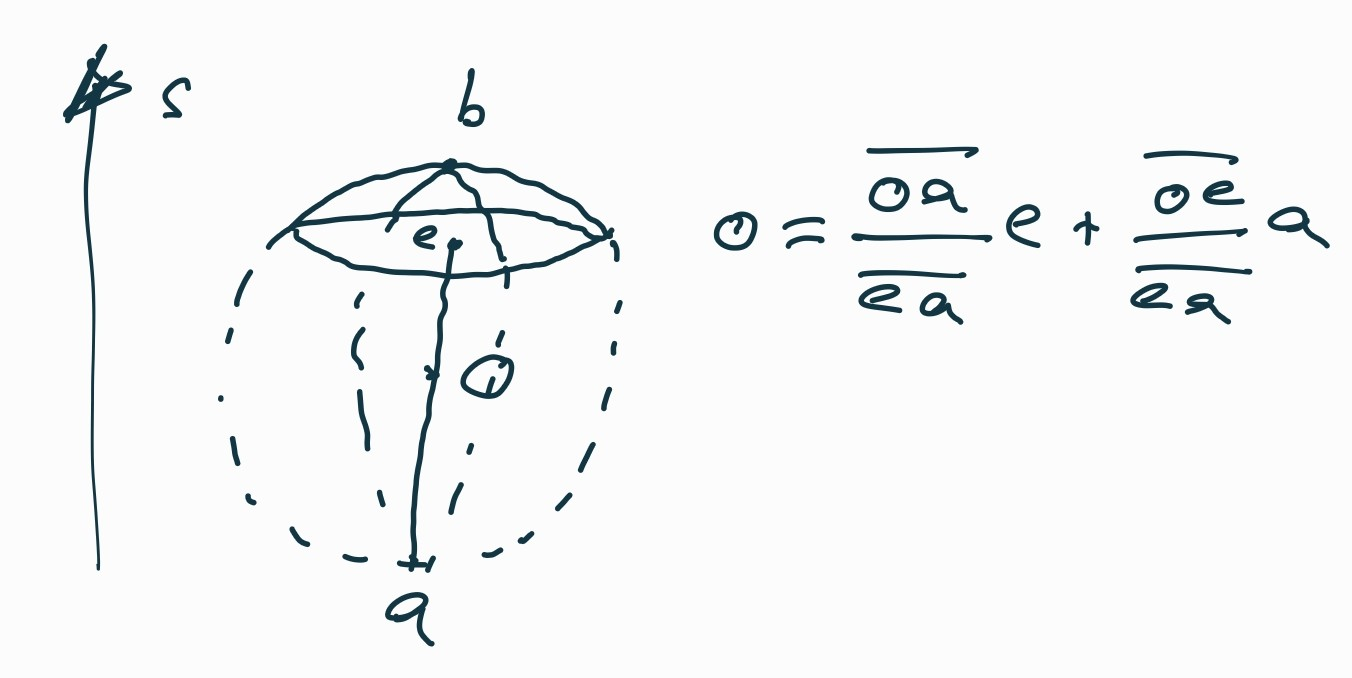
\includegraphics[width=0.8\columnwidth]{ChoquetCalculation2.jpg}
	\caption{...}
\end{figure}

In this case, the hull of $A(s)$ is the top spherical cap. We need to consider all possible convex combinations $\ens[o] = p \ens + \bar{p} \ens[c]$ where $\ens$ is in the spherical cap and $\ens[c]$ is not, and find the one with highest $p$. Since, for combinations along the same direction, $p$ increases as $\ens$ gets closer to $\ens[o]$ and as $\ens[c]$ gets further, $\ens[c]$ will be an extreme point on the lower hemisphere while $\ens$ will be on the disc at constant $s$, the lower side of the cap. Also note that the distance between $\ens[o]$ is the same for all extreme points, therefore, to maximize $p$, we simply need to minimize the distance between $\ens[o]$ and $\ens$. Therefore $\ens$ must be the intersection between the vertical axis and the disk, and $\ens[c]$ will coincide with $\ens[a]$. The coefficient $p$ will be given by the ratio of the distance $\overline{\ens[o]\ens[a]}$ and $\overline{\ens\ens[a]}$. Since $F$ is a linearly functional, we have
\begin{equation}
	\frac{\overline{\ens[o]\ens[a]}}{\overline{\ens\ens[a]}} = \frac{F(\ens[o])-F(\ens[a])}{F(\ens) - F(\ens[a])} = \frac{1}{2} \frac{b - a}{s-a}.
\end{equation}

To recap, we have (TODO: add a graph)
\begin{equation}
	\frcap_{\ens[o]}(A(s))=
	\begin{cases}
		1 & \text{if } s\leq \frac{1}{2} a + \frac{1}{2} b\\
		\frac{1}{2} \frac{b - a}{s-a} & \text{if } \frac{1}{2} a + \frac{1}{2} b < s \leq b\\
		0 & \text{if } s > b.
	\end{cases}
\end{equation}
We can now calculate the integral
\begin{equation}
	\begin{aligned}
		(C)&\int F d\frcap_{\ens[o]} := 
		\int_{-\infty}^0
		(\frcap_{\ens[o]} (A(s))-\frcap_{\ens[o]}(X))\, ds \\
		&+
		\int^\infty_0
		\frcap_{\ens[o]} (A(s))\, ds \\
		&= \int_{-\infty}^0 (1 - 1)ds + \int_{0}^{\frac{1}{2} a + \frac{1}{2} b}  1 ds \\
		&+ \int_{\frac{1}{2} a + \frac{1}{2} b}^{b}  \frac{1}{2} \frac{b - a}{s-a} ds + \int_{b}^{\infty} 0 ds \\
		&=\left[s\right]_{0}^{\frac{1}{2} a + \frac{1}{2} b}
		+ \frac{1}{2}\left(b - a\right)\left[\ln (s - a)\right]_{\frac{1}{2} a + \frac{1}{2} b}^{b} \\
		&= \frac{1}{2} a + \frac{1}{2} b + \frac{1}{2}\left(b - a\right)\left[\ln (b - a)\right. \\
		&+\left. \ln \left(\frac{1}{2} a + \frac{1}{2} b - a\right) \right] \\
		&= \frac{1}{2} a + \frac{1}{2} b + \frac{1}{2}\left(b - a\right)\ln (2)
	\end{aligned}
\end{equation}

Note that, since $\ens[o]$ is the center of the ball, $F(\ens[o]) = \frac{1}{2} a + \frac{1}{2} b \neq \frac{1}{2} a + \frac{1}{2} b + \frac{1}{2}\left(b - a\right)\ln (2)$. This means that the Choquet integral of the statistical variable with respect to the fraction capacity does not recover the expectation value.

\textbf{Space of capacities and variables.} A bigger conceptual problem is that the space of possible fraction capacities of an ensemble space depends on the ensemble space. For a classical ensemble space, for example, only additive measures are allowed. Conversely, all statistical variables are linear on the ensemble space, so the restriction on the extreme points cannot be arbitrary. In the Bloch ball case, for example, all linear functions are fully determined by two opposite points on the sphere and by two values (i.e. the eigenstates and the eigenvalues of the corresponding operator). The value for all the other points is determined.

This again corresponds to assumptions of mutual exclusivity of the extreme points and the corresponding events. As we saw before, the additivity of the measure corresponds to the ability to assign probability to a set without implicitly assigning probability to another. In terms of statistical variables, two mutually exclusive events can be assigned values independently. This, again, recovers how observable work in quantum mechanics, without mentioning quantum mechanics: only orthogonal states, that is mutually exclusive events, can be associated to measurement outcomes and be given a classical probability distribution. The non-additivity of the fraction capacity and the non-arbitrariness of the statistical variables over the extreme points, then, must be linked to the shape of the ensemble space.

Additionally, the non-additivity of the state capacity also depends on the degree of mutual exclusiveness of the events. It is additive for mutually exclusive events and sub-additive otherwise. Therefore state capacity, fraction capacity and statistical variables have to be, in a sense, compatible with each other. One may be able to use the state capacity to characterize the degree of additivity of the fraction capacity. Since in non-additive measure theory, family of capacities are often characterized the type of non-additivity,\footnote{For example, a Sugeno $\lambda$-measure is a non-additive measure $\mu$ such that $\mu(A \cup B) = \mu(A) + \mu(B) + \lambda \mu(A)\mu(B)$ for some $\lambda$ over disjoint sets $A$ and $B$. If $\lambda = 0$, the measure is additive.} this may give a way forward. Moreover, we saw that in the classical case probability measures have to be absolutely continuous with respect to the state counting measure. Maybe an elegant and meaningful compatibility condition exists between the fraction capacity and the state capacity/statistical variable that captures all requirements. Nothing along these lines came up in our literature search.


\section{Conclusion}



\section*{Acknowledgments}
This paper is part of the ongoing \textit{Assumptions of Physics} project \cite{aop-book}, which aims to identify a handful of physical principles from which the basic laws can be rigorously derived. This article was made possible through the support of grant \#62847 from the John Templeton Foundation.


\bibliography{bibliography}

\newcommand{\pj}[1] {\underbar{$#1$}}


\end{document}
